\chapter{Quark/hybrid stars}

\TODO{titles}

\TODO{units, $\hbar = c = G = k_B = 1$ or not?}

\TODO{organize project and master thesis together}

\section{Electric charge neutrality and chemical equilibrium in stars}

\TODO{generally, see Halvor's detailed discussion about this}

When we solved the Tolman-Oppenheimer-Volkoff equations for ideal neutron stars in \cref{chap:nstars}, our lives were quite simple.
The stars consisted of only one charge neutral particle, and we simply eliminated its chemical potential to find the equation of state.
Now we will consider stellar models with a greater variety of particles and non-zero electric charge.

How do we now find the equation of state, when there is one chemical potential for each kind of particle?
The answer is to impose additional physical requirements of electric charge neutrality and chemical equilibrium.
With these conditions, we will relate all but one of the chemical potentials to each other, leaving only one independent variable that we will eliminate to find the equation of state.

\subsection{Global electric charge neutrality}

We can make a very simple classical argument for why there can be no \emph{global} net electric charge in stars by comparing Newton's law of gravity and Coulomb's law.
Consider a test particle of mass $m$ and electric charge $q$ on the surface $R$ from the center of a star with total mass $M$ and electric charge $Q$.
In an idealized situation, the test particle is affected by the gravitational and electrostatic force, so that the total outwards \TODO{radial?} force on it is
\begin{equation}
	F_\text{out} = -G \frac{M m}{R^2} + k_e \frac{Q q}{R^2} .
\end{equation}
Furthermore, suppose the star consists of $N$ particles weighing \TODO{weight $\rightarrow$ mass} no more than some heavy baryon with mass $m_B$, so $M < N M_B$ and $m < m_B$.
Any electrically charged particle has about one elementary charge $q \approx \pm e$.
If the star has an opposite charge $Q = \mp Z e$, then $F_\text{out} < 0$ and the test particle stays in the star.
On the other hand, if the star has a like charge $Q = \pm Z e$, then
\begin{equation}
	F_\text{out} > -G \frac{N m_B^2}{R^2} + k_e \frac{Z e^2}{R^2} .
\end{equation}
We then surely have $F_\text{out} > 0$, provided that the number of elementary charges per particle satisfies
\begin{equation}
	\frac{Z}{N} > \frac{G m_B^2}{k_e e^2} \approx 10^{-37} ,
\end{equation}
where we have assumed a typical baryon mass $m_B = m_p = \SI{1.67e-27}{\kilogram}$.
This corresponds to practically zero electric charge per particle in the star.

This means that particle are expelled from the star while $Z > 10^{-37} N$ until $Z$ has fallen to \emph{at least} $Z < 10^{-37} N$.
We conclude that for all practical purposes, stars are \emph{globally} electrically charge neutral.

\TODO{what about radius $r < R$ instead of $r=R$?}

\TODO{what about general relativity instead of Newtonian gravity?}

\TODO{what about contribution from pressure and other things to $F_\text{out}$?}

\TODO{can I recast inequality in charge per solar mass? see discussion at beginning of \url{www.if.ufrgs.br/hadrons/MMalheiro.pdf}}

\subsection{Local electric charge neutrality}

\TODO{non-understandable comment from Møte 4, Gibbs/Maxwell contstruction etc?}

\TODO{Glendenning has papers regarding local charge neutrality (?)}

The argument in the previous section shows that a star can have no \emph{total} electric charge, but it places absolutely no limitations on its \emph{distribution}.
Moreover, our approach to calculating equations of state is inherently \emph{local} -- we obtain the equation of state $\epsilon(P)$ by eliminating the density $n$ at any \emph{single point} from the energy density $\epsilon(n)$ and pressure $P(n)$.
To make use of electric charge neutrality in our approach, we will promote it from a \emph{global} constraint to a \emph{local} one.

\TODO{now explain...}

\TODO{TOV equation is derived by assuming ideal fluid in equilibrium -- would local charge destroy that?}

\TODO{draw inspiration from standard argument that $\vec{E} = 0$ everywhere inside a conductor?}

Satisfied by
\begin{equation}
	\sum_p q_p \, n(\mu_p) = 0 ,
\end{equation}
where the sum is over all particles present, each with electric charge $q_p$.
In the zero-temperature approximation with the density \eqref{eq:nstars:density_zeroT}, this is satisfied if
\begin{equation}
	\sum_p q_p \left( \mu_p^2 - m_p^2 \right)^{3/2} = 0 .
\end{equation}

\subsection{Chemical equilibrium}

\TODO{introduce}

Important reactions
\begin{subequations}
\begin{align}
	d     &\leftrightarrow u + e + \bar{\nu}_e, \\
	s     &\leftrightarrow u + e + \bar{\nu}_e, \\
	s + u &\leftrightarrow u + d .
\end{align}
\end{subequations}
Assume neutrinos leave star \TODO{why?}.
Then chemical equilibrium implies
\begin{subequations}
\begin{align}
	\mu_d &= \mu_u + \mu_e, \\
	\mu_s &= \mu_u + \mu_e, \\
	\mu_s &= \mu_u .
\end{align}
\end{subequations}
(the third follows automatically from the two first)

\section{Linear sigma model}

\begin{figure}
\centering
\tikzsetnextfilename{potential}
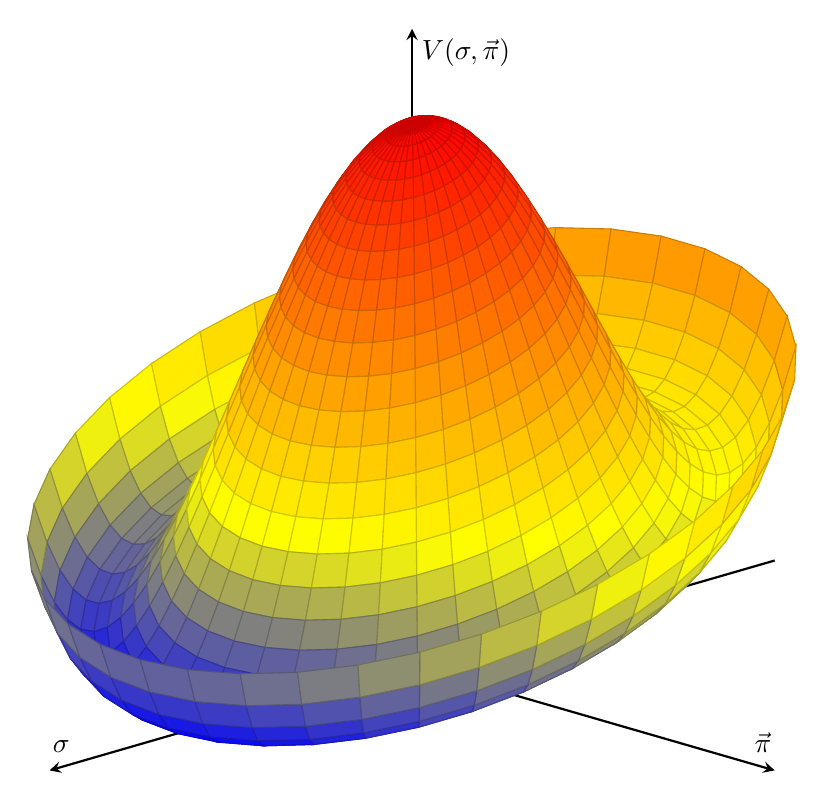
\begin{tikzpicture}
\begin{axis}[
	width = 20cm, height=15cm,
	%title = {Potential},
	xlabel = $\sigma$, ylabel = $\vec\pi$, zlabel = {$V(\sigma,\vec\pi)$},
	xmin=-4.0, xmax=+4.0, ymin=-4.0, ymax=+4.0, zmin=0, zmax=2.2,
	xtick=\empty, ytick=\empty, ztick=\empty,
	axis lines=center,
	axis line style = thick,
	view={135}{25},
	%colormap/blackwhite, mesh/interior colormap name=plasmarev,
]
	\addplot3 [surf, thin, domain=0:3.0, domain y=0:2*pi, samples=30, samples y=40, z buffer=sort] ({x*cos(deg(y))},{x*sin(deg(y))},{-1/2*((x*cos(deg(y)))^2+(x*sin(deg(y)))^2) + 1/24*((x*cos(deg(y)))^2+(x*sin(deg(y)))^2)^2 + 3/2 - 0.15*x*cos(deg(y)) + 0.15*sqrt(6)});
	%\addplot3 [domain=0:2*pi, samples=50, samples y=1] ({sqrt(6)*cos(deg(x))},{sqrt(6)*sin(deg(x))},{0});
\end{axis}
\end{tikzpicture}
\caption{\label{fig:lsm:potential}%
	With $h \neq 0$, the potential \eqref{eq:lsm:potential} looks like a tilted Mexican hat with a global minimum at $\sigma = \sqrt{6 m^2 / \lambda}, \, \vec\pi = 0$ \TODO{NO!}.
	If $h = 0$, it would rather look like an upright hat with a continuous range of minima around the brim $\sigma^2 + \vec\pi^2 = 6 m^2 / \lambda$.
	\TODO{mention this only visualizes $O(2)$}
}
\end{figure}

\TODO{justify this effective MODEL from QCD}

The Lagrangian density for the linear sigma model coupled to quarks is
\begin{equation}
	\lagr = \sum_{c=1}^{N_c} \bar{q}_c \Big[ i \slashed\partial + \mu \gamma^0 - g \left( \sigma + i \gamma^5 \vec\tau \cdot \vec\pi \right) \Big] q_c
	      + \frac12 \left[ \left( \partial_\mu \sigma \right)^2 + \left( \partial_\mu \vec\pi \right)^2 \right] - \pot(\sigma,\vec\pi) ,
\label{eq:lsm:lagrangian}
\end{equation}
\TODO{should I have $h \sigma$, too? YES!}
with the potential
\begin{equation}
	\pot(\sigma,\vec\pi) = -\frac12 m^2 \left( \sigma^2 + \vec\pi^2 \right) + \frac{\lambda}{4!} \left( \sigma^2 + \vec\pi^2 \right)^2 - h \sigma .
	                     % = \frac{\lambda}{4!} \left( \sigma^2 + \vec\pi^2 - \frac{6m^2}{\lambda} \right)^2 -\frac{3 m^4}{2 \lambda} .
\label{eq:lsm:potential}
\end{equation}
Here $q_c = (u_c, d_c)^T$ represents quarks of the $N_c = 3$ colors red, green and blue and the $N_f = 2$ flavors up and down, so $(q_c)_f$ make up a total of $N_c \times N_f = 6$ Dirac spinors.
In addition, $\sigma$ and $\vec\pi = [\pi^+, \pi^0, \pi^-]^T$ are four bosonic scalar fields representing sigma and pion mesons.
At this point, the quarks are massless Dirac fermions whose conserved charge densities $j^0 = \bar\psi \gamma^0 \psi$ are coupled to chemical potentials $\mu = \diag(\mu_u, \mu_d)$, interacting with a Yukawa coupling of strength $g$ that models the strong force \TODO{non-mentioned comment in Møte 4}, where $\vec\tau$ are the Pauli matrices \eqref{eq:tft:pauli_matrices}.
The mesons have ``imaginary mass'' $\sqrt{-m^2} = i m$ and feature a $\lambda \phi^4$-coupling.
\TODO{write $(\sigma, \vec\pi)^T$ as 4-vector and mention $O(4)$ symmetry, explain from $SU(2)_L$, $SU(2)_R$, etc.?}

To make sense of this theory, we must investigate how it behaves around the classical ground state of the potential \eqref{eq:lsm:potential}.
As shown in \cref{fig:lsm:potential}, the potential is shaped like a tilted Mexican hat with a classical ground state at $\sigma = \avg{\sigma} \neq 0$ and $\pi = \vec\pi = 0$.
Hence, the value of $\avg{\sigma}$ is determined implicitly by
\begin{equation}
	\pdv{\pot}{\sigma}_{(\sigma,\vec\pi)=(\avg{\sigma},\vec{0})} = -m^2 \avg{\sigma} + \frac{\lambda}{6} \avg{\sigma}^3 - h = 0 .
\label{eq:lsm:ground_state_implicit}
\end{equation}
We account for quantum fluctuations around the classical ground state by shifting
\begin{equation}
	\sigma \rightarrow \Avg{\sigma} + \tilde{\sigma}
	\qquad \text{and} \qquad
	\vec\pi \rightarrow \Avg{\vec\pi} + \tilde{\vec\pi}.
\end{equation}
In terms of the new fields $\tilde\sigma$ and $\tilde{\vec\pi}$, the Lagrangian \eqref{eq:lsm:lagrangian} is now
\begin{equation}
	\lagr = \sum_{c=1}^{N_c} \bar{q}_c \Big[ i \slashed\partial - m_q + \mu \gamma^0 - g \left( \tilde{\sigma} + i \gamma^5 \vec\tau \cdot \vec\pi \right) \Big] q_c
	      + \frac12 \left[ \left( \partial_\mu \tilde{\sigma} \right)^2 + \left( \partial_\mu \tilde{\vec\pi} \right)^2 \right] - \tilde{\pot}(\tilde{\sigma},\tilde{\vec\pi}) , %\pot(\avg{\sigma}+\tilde{\sigma},\avg{\vec\pi}+\tilde{\vec\pi}) ,
\end{equation}
where the quark fields $q$ have acquired effective masses
\begin{equation}
	m_q = g \avg{\sigma} .
\label{eq:lsm:mass_quark}
\end{equation}
The potential up to second order in the shifted fields is
\begin{equation}
\begin{split}
	\tilde{\pot}(\tilde{\sigma},\tilde{\vec\pi}) &= \pot(\avg{\sigma}+\tilde{\sigma},\avg{\vec\pi}+\tilde{\vec\pi}) \\
	                                             &\taylor -\frac12 m^2 \avg{\sigma}^2 + \frac{\lambda}{4!} \avg{\sigma}^4 - h \avg{\sigma} + \frac12 m_\sigma^2 \sigma^2  + \frac12 m_\pi^2 \vec\pi^2 ,
	%V(\sigma, \vec\pi) \taylor -\frac12 m^2 \avg{\sigma}^2 + \frac{\lambda}{4!} \avg{\sigma}^4 + \frac12 (\sqrt{2} m)^2 \sigma^2 .
	%V(\sigma, \vec\pi) \taylor -\frac{3 m^4}{2 \lambda} + \frac12 (\sqrt{2} m)^2 \sigma^2 .
\label{eq:lsm:potential_shifted}
\end{split}
\end{equation}
where the $\sigma$ and $\vec\pi$ fields have acquired the effective masses
\begin{subequations}
\begin{align}
	m_\sigma^2 &= \pdv[2]{\pot}{\sigma}_{(\sigma,\vec\pi)=(\avg{\sigma},\vec{0})} = -m^2 + \frac{\lambda}{2} \avg{\sigma}^2 \equalexplabove{\text{by \eqref{eq:lsm:ground_state_implicit}}} \frac{3h}{\avg{\sigma}} + 2 m^2 , \label{eq:lsm:mass_sigma} \\
	m_\pi^2    &= \pdv[2]{\pot}{\pi   }_{(\sigma,\vec\pi)=(\avg{\sigma},\vec{0})} = -m^2 + \frac{\lambda}{6} \avg{\sigma}^2 \equalexplbelow{\text{by \eqref{eq:lsm:ground_state_implicit}}} \frac{h}{\avg{\sigma}} , \label{eq:lsm:mass_pi}
\end{align}
\end{subequations}
The linear sigma model is an effective low-energy model of quantum chromodynamics, so accordingly we should take it seriously only in terms of the shifted fields around the stable ground states, and not in terms of the unshifted fields around the unstable equilibrium at the top of the Mexican hat.

Although we have and will continue to assume $h \neq 0$ in general, this is an excellent time to reflect upon the special case $h = 0$.
In this case, the potential \eqref{eq:lsm:potential} is symmetric under rotations in $O(4)$ of the field vector $(\sigma, \vec\pi)^T$.
This corresponds to movement along the ``brim'' of \emph{continuous} minima satisfying $\sigma^2 + \vec\pi^2 = 6 m^2 / \lambda$ in a flattened Mexican hat in \cref{fig:lsm:potential}.
\TODO{number of generators $=$ number of massless Goldstone bosons, $O(4)$ or $SO(4)$}
Upon choosing \emph{one} minima where $\sigma = \avg{\sigma} \neq 0$ and $\vec\pi = \avg{\vec\pi} = 0$, the symmetry would be broken to rotations of only the three $\vec\pi$ fields, and three massless Goldstone bosons would appear.
With $h \neq 0$, however, the $O(4)$ symmetry is explicitly broken, and \cref{eq:lsm:mass_pi} says $h = m_\pi^2 \avg{\sigma}$.
This is essentially Goldstone's theorem -- if $h = 0$, then $m_\pi = 0$ to ensure $\avg{\sigma} \neq 0$; but if $h \neq 0$, then $m_\pi \neq 0$.
Moreover, the smaller the value of $h$, the smaller the value of $m_\pi$, so the if $h$ is \emph{small}, the spontaneous symmetry breaking is \emph{approximate}, and the $\vec\pi$ fields are \emph{light}, but not massless.
\TODO{refine this messy paragraph}

We determine the four parameters $g$, $h$, $m$ and $\lambda$ in the original Lagrangian \eqref{eq:lsm:lagrangian} by comparing the four \emph{effective} quantities $\avg{\sigma}$, $m_\pi$, $m_\sigma$ and $m_q$ to the measurements
\begin{subequations}
\begin{alignat}{2}
	\avg{\sigma} &= \SI{93}{\mega\electronvolt}  &\qquad& \text{(\TODO{source})}, \\
	m_\pi        &= \SI{138}{\mega\electronvolt} &\qquad& \text{(\TODO{source})}, \\
	m_\sigma     &= \SI{550}{\mega\electronvolt} &\qquad& \text{(in range $\SI{400}{\mega\electronvolt} < m_\sigma < \SI{700}{\mega\electronvolt}$, by \cite{ref:pdg_review_2021})}, \\
	m_q          &= \SI{300}{\mega\electronvolt} &\qquad& \text{(by)}.
\end{alignat}
\end{subequations}
Thus, the parameters are
\begin{subequations}
\begin{alignat}{3}
	g       &= \frac{m_q}{\avg{\sigma}}                                           &&= \SI{3.23}{}                            &\qquad& \text{(by \eqref{eq:lsm:mass_quark})} , \\
	h       &= m_\pi^2 \avg{\sigma}                                               &&= \SI{1771092}{\mega\electronvolt\cubed} &\qquad& \text{(by \eqref{eq:lsm:mass_pi})} , \\
	m       &= \sqrt{\frac12 \left( m_\sigma^2 - \frac{3h}{\avg{\sigma}} \right)} &&= \SI{350}{\mega\electronvolt}           &\qquad& \text{(by \eqref{eq:lsm:mass_sigma})} , \\
	\lambda &= \frac{6}{\avg{\sigma}^3} \left( h + m^2 \avg{\sigma} \right)       &&= \SI{98}{}                              &\qquad& \text{(by \eqref{eq:lsm:ground_state_implicit})} .
\end{alignat}
\end{subequations}

According to what we learned in \cref{chap:tft} in \cref{eq:tft:boson_partition_function_momentum_out} and \eqref{eq:tft:dirac_partition_function_first},
the exact partition function corresponding to this theory is obtained by a path integral over periodic bosonic fields and anti-periodic fermionic fields, weighted by a Euclidean action in imaginary time:
\begin{equation}
	Z = \oint_- \pathintdif \bar{q} \oint_- \pathintdif q \oint_+ \pathintdif \sigma \oint_+ \pathintdif \vec\pi \exp \left\{ \int_0^\beta \dif \tau \int_V \dif^3 x \, \lagr_E[\bar{q}, q, \sigma, \vec\pi]  \right\} .
\end{equation}
As before, we are interested in $\log Z$ so we can calculate the thermodynamic quantities \eqref{eq:tft:average_quantities} and ultimately an equation of state $\epsilon(P)$, so we can solve the Tolman-Oppenheimer-Volkoff equation \eqref{eq:tov:tovsys}.
Here we will account for quantum effects of the quarks by treating them up to quadratic order (or one-loop),
but calculate only to zeroth order (or tree-level) in the meson fields and hence consider them only at the classical level.
\TODO{this is an \emph{exact} approximation as $N_c \rightarrow \infty$, because in the $\log Z$ we find below, the boson terms are $\propto N_c^0$, while the quark terms are $\propto N_c^1$}
The partition function then reads
\begin{equation}
\begin{split}
	Z &\taylor \oint_- \pathintdif \bar{q} \oint_- \pathintdif q \exp \left\{ \int_0^{\beta} \dif \tau \int_V \dif^3 x \left[ \sum_{c=1}^{N_c} \bar{q}_c \left( i \slashed\partial -m_q + \mu \gamma^0 \right) q_c + \frac12 m^2 \avg{\sigma}^2 - \frac{\lambda}{4!} \avg{\sigma}^4 + h \avg{\sigma} \right] \right\} \\
	  &=       \prod_{f=1}^{\smash{N_f}} \prod_{c=1}^{\smash{N_c}} \oint_- \pathintdif \bar{q}_f^c \oint_- \pathintdif q_f^c \\
	  &\times  \exp \left\{ \int_0^{\beta} \dif \tau \int_V \dif^3 x \left[ \sum_{f=1}^{\smash{N_f}} \sum_{c=1}^{N_c} \bar{q}_f^c \left( i \slashed\partial - m_q + \mu_f \gamma^0 \right) q_f^c + \frac12 m^2 \avg{\sigma}^2 - \frac{\lambda}{4!} \avg{\sigma}^4 + h \avg{\sigma} \right] \right\}.
\end{split}
\end{equation}
The two last terms in the exponential are independent of the fields, so
\begin{equation}
\begin{split}
	\log Z &= \frac12 \beta V m^2 \avg{\sigma}^2 - \frac{\lambda}{4!} \beta V \avg{\sigma}^4 + \beta V h \avg{\sigma} \\
	       &+ \sum_{f=1}^{N_f} \sum_{c=1}^{N_c} \log \oint_- \pathintdif \bar{q}_f^c \oint_- \pathintdif q_f^c \exp \left\{ \int_0^\beta \dif \tau \int_V \dif^3 x \, \bar{q}_f^c (i \slashed\partial + \mu_f \gamma^0 - m_q) q_f^c \right\} .
\end{split}
\end{equation}
We have already calculated the path integral in the last term from \cref{eq:tft:dirac_partition_function_first} to \cref{eq:tft:dirac_partition_function}!
Here, we get an additional factor $\sum_{c=1}^{N_c} = N_c$ from the color sum because the summand is independent of $c$,
while the flavor sum $\sum_{f=1}^{\smash{N_f}}$ yields $N_f$ terms that differ only by the unique chemical potentials $\mu_f$ associated with each quark flavor. 
Thus, we obtain
\begin{equation}
\begin{split}
	\log Z &= \frac12 \beta V m^2 \avg{\sigma}^2 - \frac{\lambda}{4!} \beta V \avg{\sigma}^4 + \beta V h \avg{\sigma} \\
	       &+ 2 V N_c \sum_{f=1}^{N_f} \int \frac{\dif^3 p}{(2 \pi)^3} \left\{ \beta E(\vec{p}) + \log \left[ e^{-\beta (E(\vec{p}) - \mu_f)}+1 \right] + \log \left[ e^{-\beta (E(\vec{p}) + \mu_f)} + 1\right] \right\} ,
\end{split}
\label{eq:lsm:potential_divergent_logz0}
\end{equation}
where the dispersion \TODO{comment Møte 4?} relation is now
\begin{equation}
	E(\vec{p}) = \sqrt{p^2 + m_q^2} .
\end{equation}
Like in \cref{chap:nstars}, we assume that the chemical potentials are chosen so that anti-particles are more or less absent, so we drop their contribution in the last term in the second line.
From the middle term in the second line, we obtained the contribution $\log Z = \beta V P$ with the pressure \eqref{eq:nstars:pressure_zeroT} after taking the zero-temperature approximation.
\TODO{justify validity of zero-temperature approximation with the new masses? no, can really only do this in a retrospective way, since I don't know a priori what the temperature is inside an unknown quark star}
This time, however, we will renormalize the infinite vacuum contribution from the first term in the second line, instead of simply dropping it, like we did back in \cref{chap:nstars}.
Thus, we obtain
\begin{equation}
\begin{split}
	\log Z &= \frac12 \beta V m^2 \avg{\sigma}^2 - \frac{\lambda}{4!} \beta V \avg{\sigma}^4 + \beta V h \avg{\sigma} + N_c N_f \log Z_0 \\
	       &+ N_c \frac{m_q^4 \beta V}{24 \pi^2} \sum_{f=1}^{N_f} \left[ (2 x_f^3 - 3x_f) \sqrt{x_f^2 + 1} + 3 \asinh x_f \right],
\end{split}
\end{equation}
where $x_f = p_f / m_q$ are normalized Fermi momenta, $\mu_f = \smash{\sqrt{p_f^2 + m_q^2}}$ are Fermi energies and the vacuum contribution is
\begin{equation}
	\log Z_0 = 2 \beta V \int \frac{\dif^3 p}{(2 \pi)^3} \sqrt{p^2 + m_q^2 } .
\label{eq:lsm:vacuum_contribution_3dim}
\end{equation}
To renormalize the vacuum contribution, let us use dimensional regularization in the minimal subtraction scheme \TODO{?}.
In $d = 3 - 2 \epsilon$ spatial dimensions, the vacuum contribution is
\TODO{can I do this in a more ``well-defined way'' by rescaling the momentum instead, like $p' = p / \Lambda^{(1-3/d)}$ where $\unit{p} = \unit{\Lambda}$, so $\unit{\dif^d p'} = \unit{\dif^3 p}$, so $\log Z$ remains dimensionless.?}
\begin{equation}
\begin{split}
	\log Z_0 &= 2 \beta V \Lambda^{3-d} \int \frac{\dif^d p}{(2 \pi)^d} \sqrt{p^2 + m_q^2} \\
	         &= 2 \beta V \Lambda^{3-d} \frac{2 \pi^{d/2}}{\Gamma(d/2)} \int_0^\infty \frac{\dif p \, p^{d-1}}{(2 \pi)^d} \sqrt{p^2 + m_q^2} .
\end{split}
\label{eq:lsm:vacuum_contribution_ddim}
\end{equation}
\TODO{what happens to the dimensions of the potential $V$ (as consequence of requiring $\log Z$ to be dimensionless)? $V \rightarrow V \lambda^{-2\epsilon}$?}
We have also multiplied the integral by $\Lambda^{3-d}$,
where $\Lambda$ is some number with $\unit{\Lambda} = \unit{p}$,
so that $\unit{\lambda^{3-d} \dif^d p} = \unit{\dif^3 p}$ and $\log Z$ remains dimensionless in all dimensions.
There is nothing that forbids us from doing so, 
as the regulator still does its only job of reducing the new integral \eqref{eq:lsm:vacuum_contribution_ddim} to the old integral \eqref{eq:lsm:vacuum_contribution_3dim} when we send $\epsilon \rightarrow 0$,
only now in a way that is well-defined in all dimensions.
The momentum integral can be written in terms of the \emph{Beta function}
\TODO{general reference}
\TODO{state that this is analytic continuation}
\begin{equation}
	B(x,y) = \int_0^\infty \dif t \, \frac{t^{x-1}}{(1+t)^{x+y}} = \frac{\Gamma(x) \Gamma(y)}{\Gamma(x+y)}
\end{equation}
if we substitute $t = p^2/m_q^2$ with $\dif t = 2 p \dif p / m_q^2$.
We then find
\begin{equation}
\begin{split}
	\log Z_0 &= \beta V \Lambda^{3-d} m_q^{d+1} \frac{2 (4 \pi)^{-d/2}}{\Gamma\big(\frac{d}{2}\big)} \int_0^\infty \dif t \, \frac{t^{d/2-1}}{(1+t)^{-1/2}} \\
	         &= \beta V \Lambda^{3-d} m_q^{d+1} \frac{2 (4 \pi)^{-d/2}}{\Gamma\big(\frac{d}{2}\big)} \frac{\Gamma\big(\frac{d}{2}\big) \Gamma\big( \textstyle{-\frac{d+1}{2}} \big)}{\Gamma\big( \textstyle{-\frac{1}{2}} \big)} .
\end{split}
\end{equation}
We now cancel the two factors $\Gamma(d/2)$ and replace $\Gamma(-1/2) = -2\sqrt{\pi}$.
Then we insert $d = 3 - 2 \epsilon$ back and use the property $\Gamma(z) = \Gamma(z+1) / z$ twice to transport the argument of the Gamma function as close as possible to its pole at $0$,
where we use its asymptotic expansion $\Gamma(\epsilon) = 1/\epsilon + \gamma + \bigo(\epsilon)$ upon arrival.
Expanding everything to zeroth order in $\epsilon$ then yields
\begin{equation}
\begin{split}
	\log Z_0 &=       -\frac{\beta V m_q^4}{8 \pi^2} \left( 4 \pi \frac{\Lambda^2}{m_q^2} \right)^\epsilon \Gamma(-2 + \epsilon) \\
	         &\taylor -\frac{\beta V m_q^4}{16 \pi^2} \left( \frac{1}{\epsilon} + \log \frac{\Lambda^2}{m_q^2} + \frac32 - \gamma + \log 4 \pi \right) .
\end{split}
\label{eq:lsm:vacuum_contribution_final}
\end{equation}
\TODO{use MS-bar now and get rid of $\gamma$ and $4 \pi$}
With the vacuum contribution \eqref{eq:lsm:vacuum_contribution_final}, the full logarithm \eqref{eq:lsm:potential_divergent_logz0} is
\begin{equation}
\begin{split}
	\log Z &= \frac12 \beta V m^2 \avg{\sigma}^2 - \frac{\lambda}{4!} \beta V \avg{\sigma}^4 - N_c N_f \frac{\beta V m_q^4}{16 \pi^2} \left[ \frac{1}{\epsilon} + \frac{3}{2} - \gamma + \log 4 \pi + \log\left(\frac{{\Lambda}^2}{m_q^2}\right) \right] \\
	       &+ N_c \frac{m_q^4 \beta V}{24 \pi^2} \sum_{f=1}^{N_f} \left[ (2 x_f^3 - 3x_f) \sqrt{x_f^2 + 1} + 3 \asinh x_f \right] .
\end{split}
\end{equation}
This investigation has revealed that the term $-N_c N_f m_q^4 \beta V / 16 \pi^2$ is guilty of the offense of vacuum divergence.
We also see that the preceding term can shield society from this criminal if we split the coupling 
\begin{equation}
	\lambda = \lambda_P + \delta\lambda
	\qquad \text{with the counterterm} \qquad
	\delta\lambda = -N_c N_f \frac{3 g^4}{2 \pi^2 \epsilon} .
\end{equation}
Then the innocent, finite and renormalized expression for $\log Z$ is
\begin{equation}
\begin{split}
	\log Z &= \frac12 \beta V m^2 \avg{\sigma}^2 - \frac{\lambda_P}{4!} \beta V \avg{\sigma}^4 + \beta V h \avg{\sigma} - N_c N_f \frac{\beta V m_q^4}{16 \pi^2} \left[ \frac{3}{2} - \gamma + \log 4 \pi + \log\left(\frac{{\Lambda}^2}{m_q^2}\right) \right] \\
	       &+ N_c \frac{m_q^4 \beta V}{24 \pi^2} \sum_{f=1}^{N_f} \left[ (2 x_f^3 - 3x_f) \sqrt{x_f^2 + 1} + 3 \asinh x_f \right] .
\end{split}
\end{equation}
From $\log Z$, we can finally build a bridge to thermodynamics with the grand potential density
\TODO{I remove $\gamma$ and $\log 4 \pi$, use modified minimal subtraction?}
\begin{equation}
\begin{split}
	\omega = \frac{\Omega}{V} = -\frac{\log Z}{\beta V} &= -\frac12 m^2 \avg{\sigma}^2 + \frac{\lambda_P}{4!} \avg{\sigma}^4 - h \avg{\sigma} + N_c N_f \frac{m_q^4}{16 \pi^2} \left[ \frac{3}{2} + \log\left(\frac{{\Lambda}^2}{m_q^2}\right) \right] \\
	                                                    &- N_c \frac{m_q^4}{24 \pi^2} \sum_{f=1}^{N_f} \left[ (2 x_f^3 - 3x_f) \sqrt{x_f^2 + 1} + 3 \asinh x_f \right] .
\end{split}
\label{eq:lsm:grand_potential}
\end{equation}
The renormalization procedure has introduced the an unknown parameter $\Lambda$.
To determine it, we require that the minimum of the grand potential \eqref{eq:lsm:grand_potential} \emph{as a function of $\avg{\sigma}$} remains at the minimum $f_\pi = \SI{93}{\mega\electronvolt}$ of the potential \eqref{eq:lsm:potential}, defined by \eqref{eq:lsm:ground_state_implicit}, when we are in vacuum.
Then the second line of the grand potential is absent, and the first three terms already satisfies, so this is satisfied if
\begin{equation}
	\pdv*{\left[ N_c N_f \frac{m_q^4}{16 \pi^2} \left( \frac32 + \log \frac{\Lambda^2}{m_q^2} \right) \right] }{\avg{\sigma}} = 0,
	\quad \text{yielding} \quad
	\Lambda = \frac{g f_\pi}{\sqrt{e}} = \SI{182}{\mega\electronvolt}.
\end{equation}

To ensure the star is charge neutral, we take our linear sigma model coupled to quarks and place it on top of a background of electrons by modifying.
This amounts to adding one more fermion term to the Lagrangian density \eqref{eq:lsm:lagrangian} and, ultimately, the grand potential \eqref{eq:lsm:grand_potential}.
Since the electrons are so light compared to the quarks, we approximate them as massless \TODO{do properly}.
\TODO{what about their renormalized vacuum term?}
Thus,
\begin{equation}
\begin{split}
	\omega = \frac{\Omega}{V} = -\frac{\log Z}{\beta V} &= -\frac12 m^2 \avg{\sigma}^2 + \frac{\lambda_P}{4!} \avg{\sigma}^4 - h \avg{\sigma} + N_c N_f \frac{m_q^4}{16 \pi^2} \left[ \frac{3}{2} + \log\left(\frac{{\Lambda}^2}{m_q^2}\right) \right] \\
	                                                    &- \frac{\mu_e^4}{12 \pi^4} - N_c \frac{m_q^4}{24 \pi^2} \sum_{f=1}^{N_f} \left[ (2 x_f^3 - 3x_f) \sqrt{x_f^2 + 1} + 3 \asinh x_f \right] .
\end{split}
\label{eq:lsm:grand_potential}
\end{equation}

\TODO{my idea for what to do next:}
\begin{enumerate}
\item Have $\omega(\avg{\sigma}, \mu)$.
\item Must ensure that $P = 0$ in vacuum, i.e. when $n(\mu) = 0$, or $x_f = 0$ or $\mu = m$ (generally).
\item Therefore shift $\omega(\avg{\sigma},\mu) \rightarrow \omega(\avg{\sigma},\mu) - \omega(\avg{\sigma},m)$, or something along those lines.
\end{enumerate}



\TODO{determine all $4$ couplings from $4$ requirements, only use physical values $h \neq 0$ (?)}

\TODO{seems to be same as Berge got, only with different sign of $m^2$}

\TODO{things below here are unfinished}

\TODO{why renormalize vacuum? seems like it only adds minor corrections to grand potential?}

\TODO{retrace and check calculation}

\TODO{find free energy and plot it}

\TODO{add electrons? ignore their mass?}

\TODO{ignore constant terms in $\log Z$. but the $\log Z$ and thus $P$ should be $0$ when WHAT is satisfied?}

\TODO{eliminate three chemical potentials for electrons, ups, downs with electric charge neutrality and chemical equilibrium for one process, so that only one chemical potential is left?}

\TODO{subtract something from $P$ so that $P = 0$ in vacuum}

\TODO{
do I determine $\lambda P$ from
\begin{equation}
	\avg{\sigma}_\text{min} = f_\pi = \frac{\sqrt{6} m}{\sqrt{\lambda}} = \frac{\sqrt{6} m}{\sqrt{\lambda_P \left( 1 + \frac{\delta \lambda}{\lambda_p} \right)}} \taylor \frac{\sqrt{6} m}{\lambda_P}
\end{equation}
???
}

\iffalse
\begin{figure}
\tikzsetnextfilename{grand-potential}
\begin{tikzpicture}
\begin{axis}[
	xmin = 0, xmax = 200, ymin=-100, ymax=+500,
	declare function={
		Nc = 3;
		Nf = 2;
		msigma = 800;
		mpi = 0;
		mq0 = 300;
		m = sqrt(2)*msigma;
		fpi = 93;
		h = fpi * mpi^2;
		g = mq0 / fpi;
		mq(\sigma) = g * \sigma;
		lambda = 6*m^2 / fpi^2;
		Lambda = mq0 / sqrt(e);
		x(\sigma,\mu) = sqrt((\mu)^2/(mq(\sigma))^2 - 1);
		asinh(\y) = ln(\y + sqrt((\y)^2+1));
		v0(\sigma) = -1/2*m^2*(\sigma)^2 + lambda/24*(\sigma)^4 - h*\sigma; % bosonic contribution
		vr(\sigma) = Nc*Nf*(mq(\sigma))^4/(16*pi^2)*(3/2+ln(Lambda^2 / (mq(\sigma))^2)); % renormalized vacuum contribution
		vf(\sigma,\mu) = -Nc*(mq(\sigma))^4/(24*pi^2) * ( (2*(x(\sigma,\mu))^3-3*x(\sigma,\mu))*sqrt((x(\sigma,\mu))^2+1) + 3*asinh(x(\sigma,\mu)) ); % quark/flavor contribution
		v(\sigma,\mu) = v0(\sigma) + vr(\sigma); % + vf(\sigma,\mu);
	},
]
\addplot [domain=0:200] {v(x,0) / fpi^4};
\end{axis}
\end{tikzpicture}
\end{figure}
\fi

\begin{figure}
\tikzsetnextfilename{grand-potential}
\begin{tikzpicture}
\begin{axis}[
	view={135}{20},
	width=14cm, height=12cm,
	%xmin=-125, xmax=+125, ymin=250, ymax=1000, zmin=-275, zmax=0,
	%zmax=0, zmin=-500,
	zmax=4, zmin=-10,
	xlabel = {$\avg{\sigma}$}, ylabel = {$\mu$}, zlabel = {$\omega(\avg{\sigma}, \mu)$},
	colormap/blackwhite, mesh/interior colormap name=plasmarev,
	3d box=complete,
]
\addplot3 [surf, very thin, mesh/ordering=x varies] table [x=sigma, y=mu, z=omega] {../code/data/lsmpot.dat};
\addplot3 [blue] table [x=sigma, y=mu, z=omega] {../code/data/lsmpotmin.dat}; % plot line of minima
\addplot  [gray] table [x=sigma, y=mu, z expr={-10}] {../code/data/lsmpotmin.dat}; % plot its "shadow" in bottom plane
\end{axis}
\end{tikzpicture}
\caption{\label{fig:lsm:grand_potential}%
$\mu_u = \mu_d = \mu$, no electrons: phase transition
\TODO{(unfinished, something wrong?) plot $\Omega(\mu,\avg{\sigma})$, show phase transition?}
}
\end{figure}
